% !TeX root = ../../ZF_bmicha_Ana.tex
\subsection{Gradient}
    $$
        \grad(f(x,y,z)) = \begin{pmatrix}
            f_x \\ f_y \\ f_z
        \end{pmatrix}
    $$
    \begin{itemize}
        \item Steht senkrecht auf Niveauflächen/ -linien.
        \item Zeigt in Richtung des grössten Anstiegs der Funktionswerte.
    \end{itemize}
    \subsubsection{2D - $f(x,y)$}
        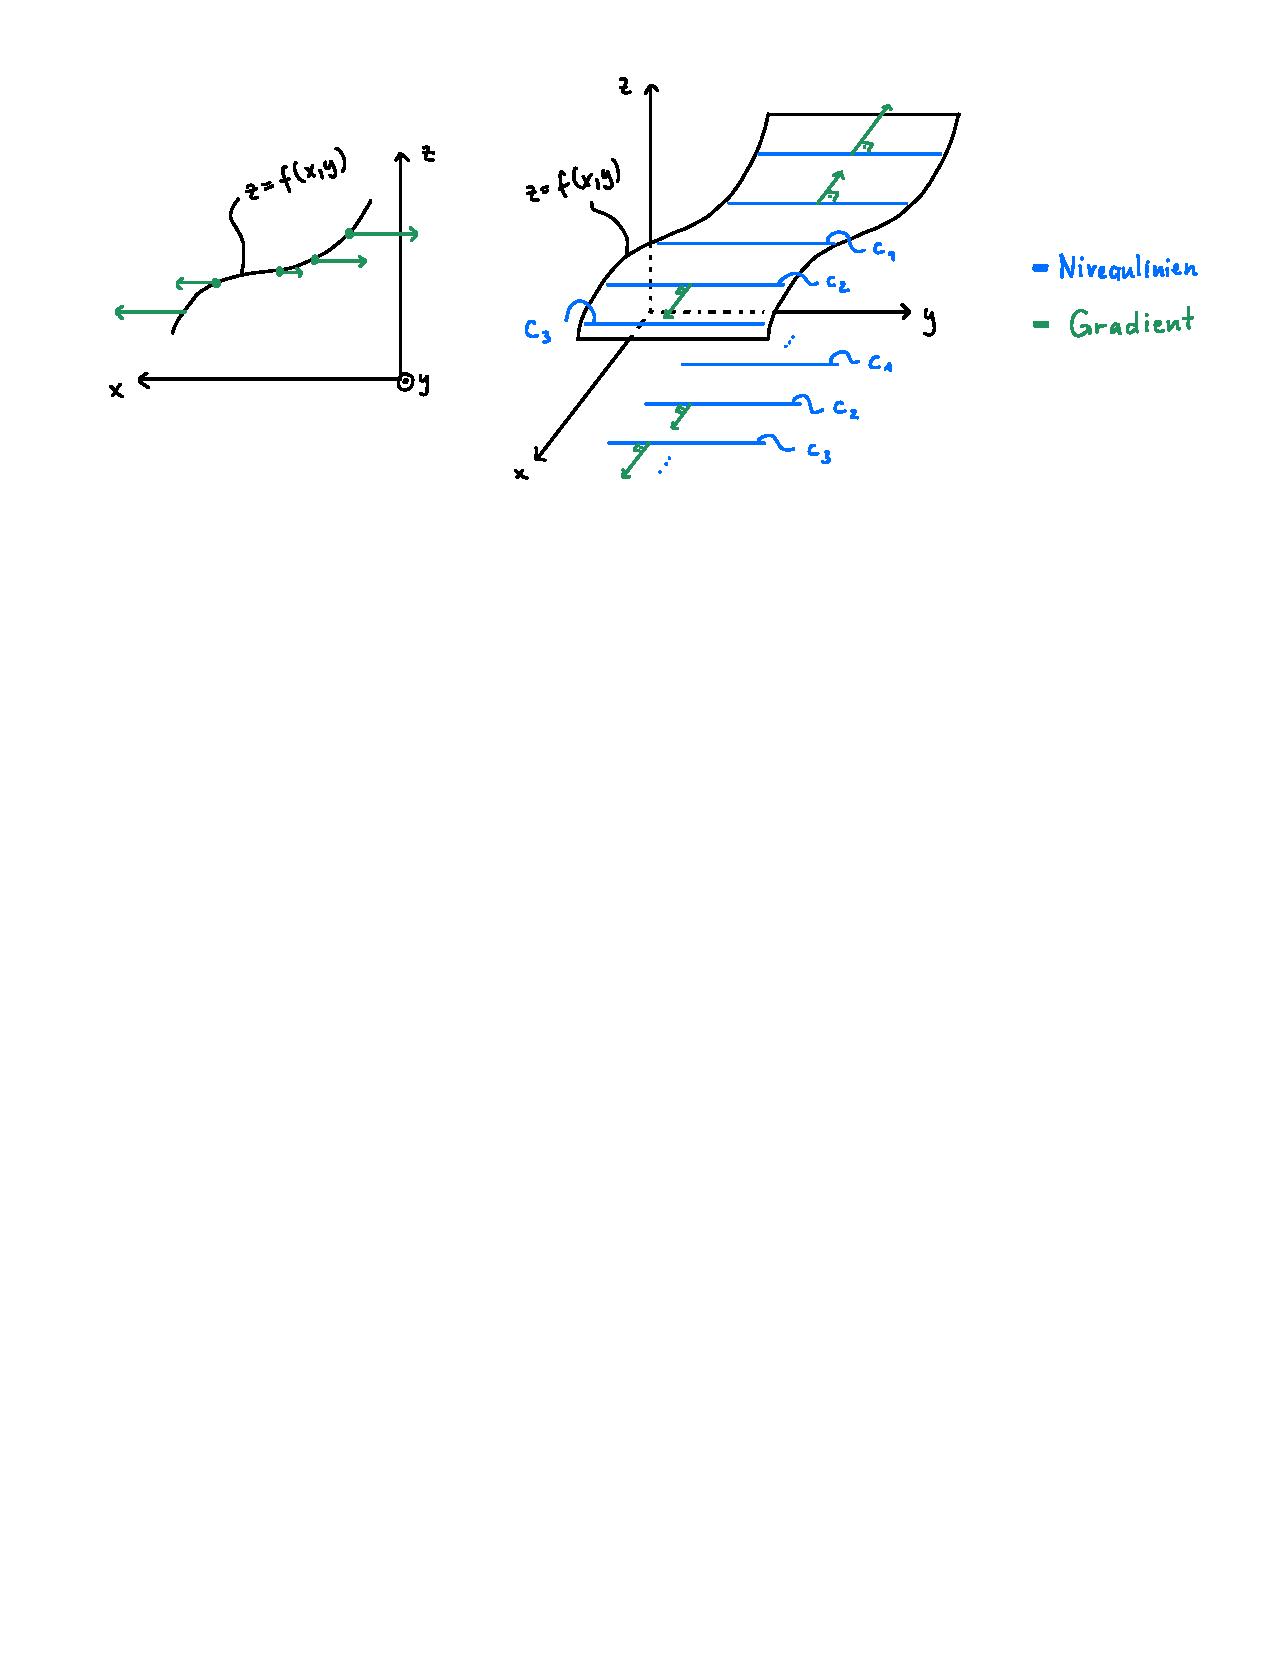
\includegraphics[width=\linewidth]{src/Mehrdimensionale-Funktionen_Differentialrechnung/grad_2D.pdf}
    \subsubsection{3D - $f(x,y,z)$}
        \begin{center}
            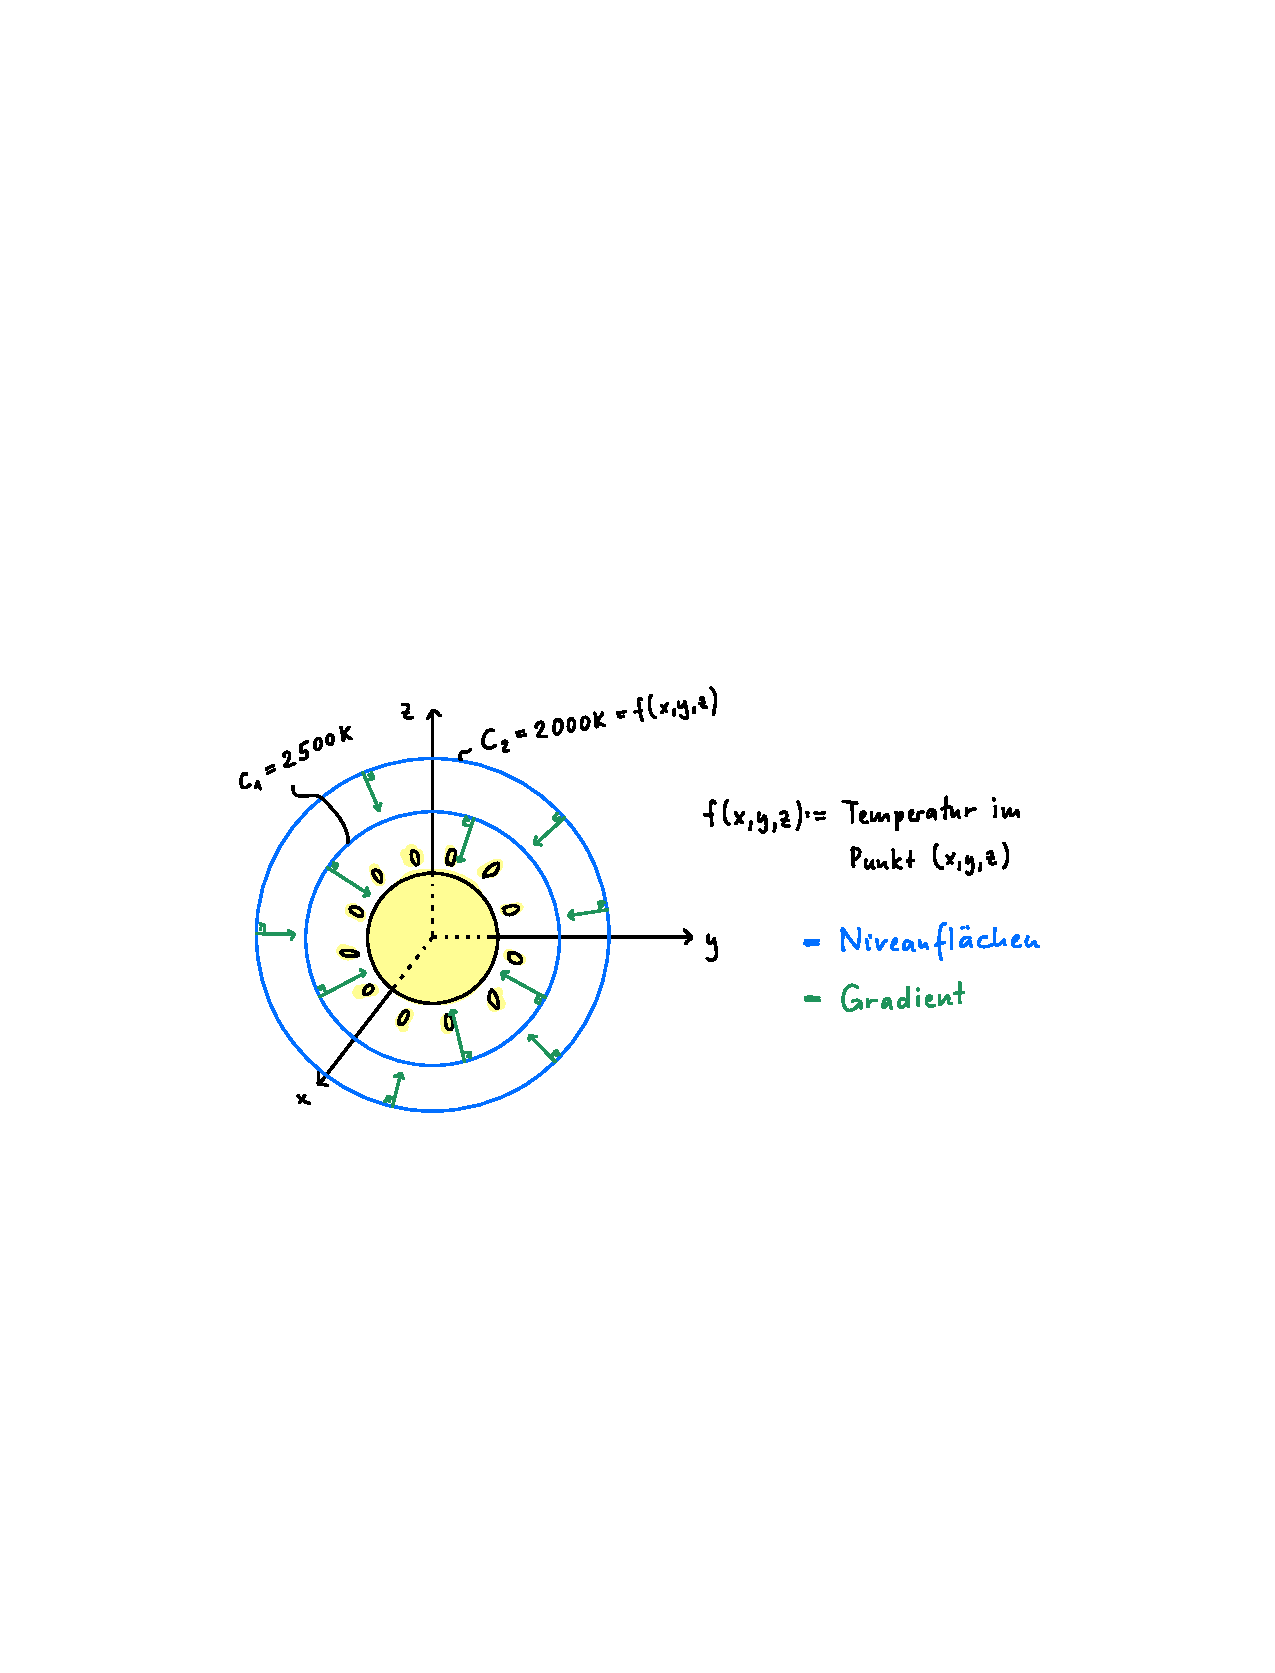
\includegraphics[width=0.8\linewidth]{src/Mehrdimensionale-Funktionen_Differentialrechnung/grad_3D.pdf}
        \end{center}